\documentclass[11pt,a4paper]{article}
\usepackage[margin=1.0in]{geometry}
\usepackage[skip=8pt plus1pt, indent=0pt]{parskip}
\usepackage[scaled]{berasans}
\renewcommand*\familydefault{\sfdefault}

\usepackage{polski}
\usepackage[T1]{fontenc}
\usepackage[utf8]{inputenc}

\usepackage{hyperref}
\usepackage{amsmath, amsthm}
\usepackage{graphicx}
\usepackage{float}
\usepackage{pgfplots}
\usepackage[color=orange!25]{todonotes}
\usepackage{listings}
\newcommand{\todoinfo}[2][]{\todo[color=green!30, #1]{#2}}
\newcommand{\deemph}[1]{{\color{black!40}{\footnotesize #1}}}


\title{Raport z laboratorium przedmiotu\\Informatyka w Medycynie\\Projekt tomografu}
\author{\emph{Ivan Kaliadzich 153936, Mikołaj Diakowski 151843}}
\date{24 marca 2024}


\begin{document}
\maketitle
    \section{Zastosowany model tomografu}
    W projekcie zdecydowaliśmy się na zastosowanie modelu tomografu stożkowego.
    \section{Zastosowany język programowania wraz z bibliotekami}
    W projekcie użyliśmy języka Python jako świetnego narzędzia do obliczeń i przetwarzania obrazów.
    Wykorzystaliśmy
    następujące biblioteki:
    \begin{itemize}
        \item \texttt{imageio} - do wczytywania obrazów
        \item \texttt{ipywidgets} - do tworzenia interaktywnych elementów
        \item \texttt{numpy} - do operacji matematycznych
        \item \texttt{pydicom} - do wczytywania obrazów w formacie DICOM
        \item \texttt{matplotlib} - do rysowania wykresów
        \item \texttt{scipy} - do przetwarzania sygnałów
        \item \texttt{skimage} - do przetwarzania obrazów
        \end{itemize}
    \section{Opis głównych funkcji programu}
    \subsection{Pozyskiwanie odczytów dla poszczególnych detektorów}
    Fragment kodu:
\begin{lstlisting}[language=Python, basicstyle=\normal, breaklines=true]
def picture2sinogram(picture, width, detector_amount, alpha):
    centre_of_image = [int(picture.shape[1]/2), int(picture.shape[0]/2)]
    r = min(centre_of_image[0], centre_of_image[1])
    print(centre_of_image)

    sinogram = []
    lines = []

    # poruszaj emiterem 360/n razy o kąt alpha i zbierz próbki promieni.
    for i in range(0, 360, alpha):
        sinogram.append([])
        lines.append([])
        for detector in range(0, detector_amount):
            x0 = r * np.cos(i * np.pi / 180)
            y0 = r * np.sin(i * np.pi / 180)

            x1 = r * np.cos((i + 180 - (width / 2) + detector * (width / (detector_amount - 1))) * np.pi / 180)
            y1 = r * np.sin((i + 180 - (width / 2) + detector * (width / (detector_amount - 1))) * np.pi / 180)

            x0 = int(x0) + np.floor(centre_of_image[1])
            x1 = int(x1) + np.floor(centre_of_image[1])
            y0 = int(y0) + np.floor(centre_of_image[0])
            y1 = int(y1) + np.floor(centre_of_image[0])

            line = bresenham_line(x0, y0, x1, y1)

            pixel = change_brightness(picture, line)


            sinogram[-1].append(pixel)
            lines[-1].append([x0, y0, x1, y1])



    return sinogram, lines
    \end{lstlisting}
    Funkcja ta przeprowadza transformację Radona na obrazie wejściowym.
    Algorytm ten pozwala jednocześnie na uśrednienie jasności punktów obrazu wynikowego, a także na jego normalizację.
    Warto zauważyć, że funkcja ta zwraca również listę linii, które są używane do rysowania obrazu wynikowego.
    \subsection{Filtracja sinogramu i zastosowany rozmiar maski}
\begin{lstlisting}[language=Python, basicstyle=\normal, breaklines=true]

def filtering_sinogram(sinogram):
    sinogram_shape = np.shape(sinogram)
    number_of_projections = sinogram_shape[0]
    number_of_detectors = sinogram_shape[1]

    filtered = np.zeros((number_of_projections, number_of_detectors))
    mask = do_mask(number_of_detectors)

    # splot każdej projekcji z naszą maską
    for projection in range(0, number_of_projections, 1):
        filtered[projection] = sig.convolve(sinogram[projection], mask, mode='same', method='direct')

    return filtered


def do_mask(detectors):
    # maska jednowymiarowa
    mask_size = math.floor(detectors / 2)
    mask = np.zeros(mask_size)
    center = math.floor(mask_size / 2)
    for i in range(0, mask_size, 1):
        k = i - center
        if k % 2 != 0:
            mask[i] = (-4 / np.pi ** 2) / k ** 2
    mask[center] = 1
    return mask
\end{lstlisting}
    Funkcja \texttt{filtering\_sinogram} przeprowadza filtrację sinogramu.
    Warto zauważyć, że funkcja ta wykorzystuje funkcję \texttt{do\_mask}, która zwraca maskę filtrującą.
    Maskę wykonaliśmy dla połowy detektorów, co pozwala na zastosowanie filtracji w dziedzinie częstotliwości.
    \subsection{Ustalanie jasności poszczególnych punktów obrazu wynikowego oraz jego przetwarzanie końcowe}

\begin{lstlisting}[language=Python, basicstyle=\normal, breaklines=true]
def back_projection(picture, sinogram, lines, filtr):
    projection = []
    if filtr:
        sinogram = filtering_sinogram(sinogram)

    picture_shape = np.shape(picture)
    width = picture_shape[0]
    height = picture_shape[1]


    sinogram_shape = np.shape(sinogram)
    number_of_projections = sinogram_shape[0]
    number_of_detectors = sinogram_shape[1]

    # dane do tworzenia gifa i statystyk
    images = []
    iterator = 0
    # dane do rekonstrukcji zdjęcia
    reconstructed_ = np.zeros(shape=picture_shape)
    helper = np.zeros(shape=picture_shape)

    # rekonstrukcja zdjęcia
    for projection in range(0, number_of_projections, 1):
        for detector in range(0, number_of_detectors, 1):
            x0, y0, x1, y1 = lines[projection][detector]
            line = bresenham_line(x0, y0, x1, y1)
            value = sinogram[projection][detector]
            for i in range(0, len(line), 1):
                x, y = line[i]
                if 0 <= x < width and 0 <= y < height:
                    reconstructed_[int(x)][int(y)] += value
                    helper[int(x)][int(y)] += 1
        images.append(reconstructed_.copy())
    return reconstructed_, images


def scale_brightness(image1):
    return rescale_intensity(image1, out_range=(0, 1))
\end{lstlisting}
    Funkcja \texttt{back\_projection} przeprowadza odwrotną projekcję na obrazie wynikowym.
    Warto zauważyć, że funkcja ta zwraca również listę obrazów, które są używane do stworzenia animacji. Funkcja \texttt{scale\_brightness} służy do skalowania jasności obrazu wynikowego.
    Wykorzystywana ona jest do tworzenia statystyk.
    \subsection{Wyznaczanie wartości miary RMSE na podstawie obrazu źródłowego oraz wynikowego}\label{sec:wyznaczanie-wartosci-miary-rmse-na-podstawie-obrazu-zrodowego-oraz-wynikowego}
    \begin{lstlisting}[language=Python, basicstyle=\normal, breaklines=true]
sinogram_without_filter, lines_without_filter = picture2sinogram(original_image, width, detector_amount, alpha)
constr_without_filter, _ = back_projection(original_image, sinogram_without_filter, lines_without_filter, False)
scale_brightness(constr_without_filter)
print(f"Mean squared error dla obrazu bez filtrowania: {math.sqrt(mean_squared_error(original_image, constr_without_filter))}")
\end{lstlisting}
    Funkcja \texttt{mean\_squared\_error} zwraca wartość miary MSE dla obrazu wynikowego oraz obrazu źródłowego.

    \subsection{Odczyt i zapis plików DICOM}
    \begin{lstlisting}[language=Python, basicstyle=\normal, breaklines=true]
import pydicom
import pydicom._storage_sopclass_uids

def create_dicom(name_patient, date_patient, commentary_patient):
    global reconstructed
    photo_dcm = (reconstructed).astype(np.uint16)

    meta = pydicom.Dataset()
    meta.MediaStorageSOPClassUID = pydicom._storage_sopclass_uids.MRImageStorage
    meta.MediaStorageSOPInstanceUID = pydicom.uid.generate_uid()
    meta.TransferSyntaxUID = pydicom.uid.ExplicitVRLittleEndian

    Data = pydicom.Dataset()
    Data.file_meta = meta
    Data.is_little_endian = True
    Data.is_implicit_VR = False
    Data.SOPClassUID = pydicom._storage_sopclass_uids.MRImageStorage
    Data.PatientName = name_patient
    Data.StudyDate = date_patient
    Data.StudyDescription = commentary_patient
    Data.Modality = "MR"
    Data.SeriesInstanceUID = pydicom.uid.generate_uid()
    Data.StudyInstanceUID = pydicom.uid.generate_uid()
    Data.FrameOfReferenceUID = pydicom.uid.generate_uid()

    Data.BitsAllocated = 16
    Data.BitsStored = 16
    Data.HighBit = 15
    Data.SamplesPerPixel = 1
    Data.ImagesInAcquisition = "1"
    Data.Rows = photo_dcm.shape[0]
    Data.Columns = photo_dcm.shape[1]

    Data.ImagePositionPatient = r"0\0\1"
    Data.ImageOrientationPatient = r"1\0\0\0\-1\0"
    Data.ImageType = r"ORIGINAL\PRIMARY\AXIAL"
    Data.RescaleIntercept = "0"
    Data.RescaleSlope = "1"
    Data.PixelSpacing = r"1\1"
    Data.PhotometricInterpretation = "MONOCHROME2"
    Data.PixelRepresentation = 1

    pydicom.dataset.validate_file_meta(Data.file_meta, enforce_standard=True)
    Data.PixelData = photo_dcm.tobytes()
    Data.save_as("DICOM.dcm")
    \end{lstlisting}
    Funkcja \texttt{create\_dicom} tworzy plik DICOM na podstawie obrazu wynikowego.
    Jako parametry przyjmuje imię i nazwisko pacjenta, datę badania oraz komentarz.

    \subsection{Przykładowy wynik działania programu}
    \begin{figure}[H]
        \centering
        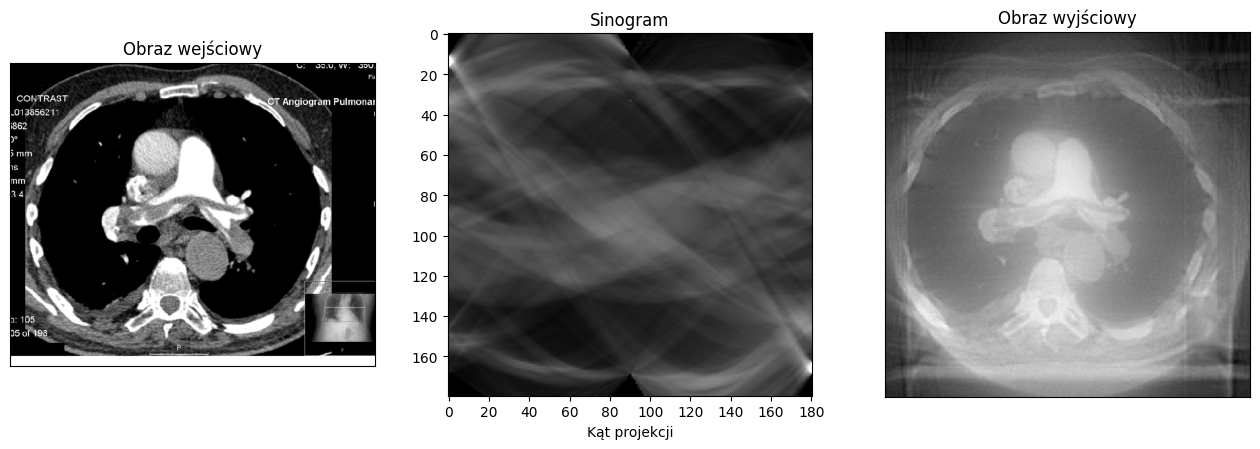
\includegraphics[width=0.8\textwidth]{inputoutput1}
        \caption{Przykładowy wynik działania programu -- bez filtrowania}
    \end{figure}

    \begin{figure}[H]
        \centering
        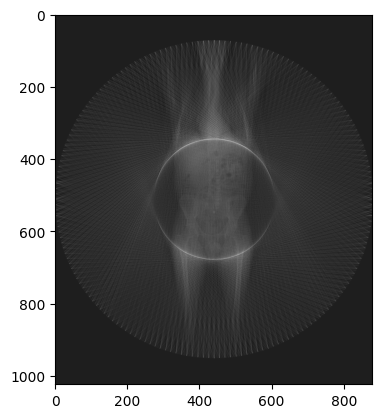
\includegraphics[width=0.8\textwidth]{inputoutput2}
        \caption{Przykładowy wynik działania programu -- z filtrowaniem}
    \end{figure}
    \section{Statystyki}
    \begin{figure}[H]
        \centering
        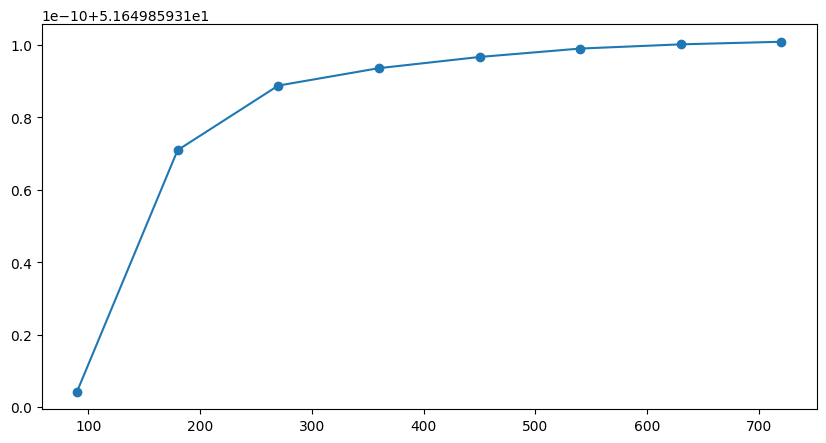
\includegraphics[width=0.8\textwidth]{rmse_detectors}
        \caption{Wyniki miary RMSE dla różnej liczby detektorów}
    \end{figure}

    \begin{figure}{H}
        \centering
        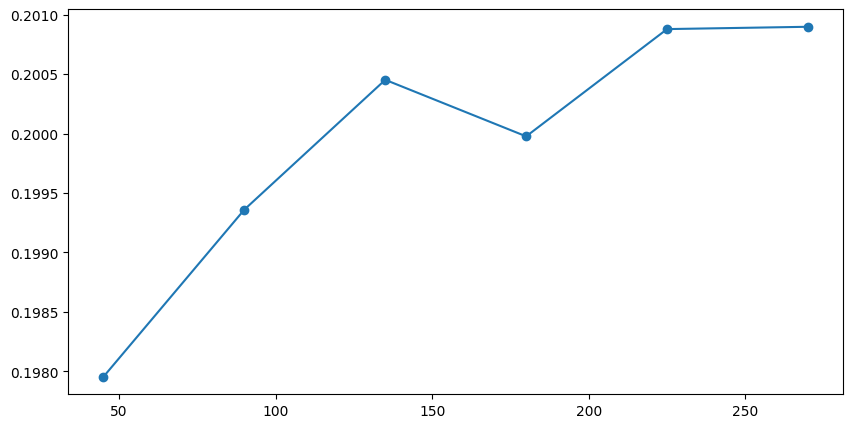
\includegraphics[width=0.8\textwidth]{mse_fan}
        \caption{Wyniki miary RMSE dla różnej rozpiętości wachlarza kątów}
    \end{figure}

    \begin{figure}[H]
        \centering
        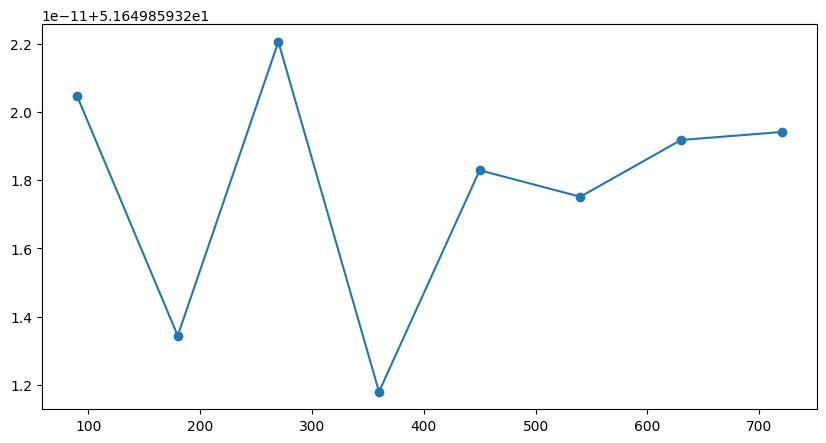
\includegraphics[width=0.8\textwidth]{mse_amount}
        \caption{Wyniki miary RMSE dla różnej liczby skanów}
    \end{figure}

    Zwiększenie liczby skanów powoduje rozrzut przypominający stabilizujący się sygnał.
    Na obrazku można zauważyć polepszenie jakości obrazu wynikowego.

    \subsection{Porównanie RMSE dla obrazu filtrowanego i niefiltrowanego}
    Mean squared error dla obrazu bez filtrowania: 13.494372974090599

    Mean squared error dla obrazu z filtrowaniem: 0.14701867613771755

    Filtracja sinogramu pozwala na znaczne zmniejszenie błędu średniokwadratowego.
\end{document}